\documentclass[11pt]{article} 
\usepackage{geometry}
\geometry{letterpaper}

\usepackage{graphicx}   
\usepackage{amssymb}
\usepackage{float}
\usepackage{tabularx}
\usepackage{framed}
\usepackage{hyperref}
\hypersetup{
    colorlinks,
    citecolor=black,
    filecolor=black,
    linkcolor=black,
    urlcolor=black
}
\usepackage{cleveref}
%\usepackage[autostyle]{csquotes}
\usepackage[english]{babel}
\usepackage[backend=biber,style=numeric,sorting=none]{biblatex}
\addbibresource{cites.bib}

\defbibheading{bibliography}[\refname]{}

\begin{document}

\newcommand{\PROJECTNAME}{HydroSwarm}

\begin{titlepage}
	\newcommand{\HRule}{\rule{\linewidth}{0.2mm}}
	\begin{center}
	\textsc{\LARGE McMaster University}\\[1.5cm]
	
	\textsc{\Large \PROJECTNAME}\\[0.5cm]
	\textsc{\large Software \& Mechatronics Capstone}\\[0.5cm] 

	\HRule\\[0.4cm]
		{\huge\bfseries Requirements Document}\\[0.4cm]
	\HRule\\[0.4cm]
	
	\begin{minipage}[t][][t]{0.5\textwidth}
		\begin{flushleft} \large
			\emph{Authors:}\\
			Victor Velechovsky \\
			Amandeep Panesar \\
			Taha Mian \\
			Gabriel Potter \\
			Nishanth Balamohan \\
		\end{flushleft}
	\end{minipage}
	~
	\begin{minipage}[t][][t]{0.4\textwidth}
		\begin{flushright} \large
			\emph{Professor:} \\
			Dr. Alan Wassyng \\[0.4cm]
			\emph{Teaching Assistants:} \\
			Nicholas Annable \\
			Joshua Barkovic \\
			Spencer Deevy \\
			Viktor Smirnov
		\end{flushright}
	\end{minipage}\\[2cm]
	
	
\includegraphics[width=0.3\textwidth]{images/logo.png} \\
	{\large Last compiled on \today}
	\end{center}

\end{titlepage}

\tableofcontents
\listoffigures

\vfill
\begin{figure}[htbp]
   \centering
   \noindent\begin{tabularx}{\textwidth}{| >{\centering\arraybackslash}m{0.2\textwidth} | >{\centering\arraybackslash}m{0.2\textwidth} | >{\centering\arraybackslash}m{0.2\textwidth} | >{\centering\arraybackslash}m{0.285\textwidth} |}
   \hline 
   \textbf{Date} & \textbf{Revision} & \textbf{Comments} & \textbf{Author(s)} \\
   \hline
   Oct 28/2018 & 0 & Basic template & All authors\\ \hline
   Oct 29/2018 & 1 & Functional Requirements Added & All authors\\ \hline
   Oct 30/2018 & 2 & Other sections added & All authors\\ \hline
   Oct 31/2018 & 3 & Final draft for Requirements Deadline & All authors\\ \hline
   \end{tabularx}
   \caption{Revision History}
\end{figure}

\newcommand{\functionalRequirement}[7]{
\begin{framed}
	\noindent\textbf{Requirement ID}: F{#1} \hfill \textbf{Requirement Type}: F \hfill\\\\
	\noindent\textbf{Description}: {#2} \\
	\textbf{Rationale}: {#3} \\
	\textbf{Fit Criterion}: {#4} \\
	\textbf{Originator}: {#5} \\
	\textbf{Priority}: {#6} \hfill \\
	\noindent\textbf{History}: {#7}
\end{framed}
}

\newcommand{\nonFunctionalRequirement}[7]{
\begin{framed}
	\noindent\textbf{Requirement ID}: NF{#1} \hfill \textbf{Requirement Type}: NF \hfill\\\\
	\noindent\textbf{Description}: {#2} \\
	\textbf{Rationale}: {#3} \\
	\textbf{Fit Criterion}: {#4} \\
	\textbf{Originator}: {#5} \\
	\textbf{Priority}: {#6} \hfill \\
	\noindent\textbf{History}: {#7}
\end{framed}
}

\newpage
%THIS DOCUMENT MUST INCLUDE
%-Scope
%-Context Diagram showing boundaries---???
%-Monitored and controller variables (with units)
%-Constraints
%-Behavior overview including notation---???
%-Diagrams showing functional decomposition---???
%-Required behavior description (keep away from design as much as possible)
%-Rationale where necessary - includes simulation analysis if you have any
%-Performance requirements
%-Normal operation (optional if handled in requirements with undesired event handling)
%-Undesired event handling(optional if handled in requirements with normal operation) --- ???
%-List of requirements that are likely to change
%-List of requirements that are not likely to change ---???
%-References

\section{Introduction}

There are many applications for carrying out distributed measurements in large bodies of water. Weather tracking, oil spill tracking, and water toxicity measurements are among many. Unfortunately, it is both expensive and time-consuming to carry out such measurements over large regions. It typically requires many measurement stations, all placed in discrete locations, in order to provide accurate readings over large areas. We propose a fundamentally different approach.

\subsection{Project Overview}

\PROJECTNAME \space is a \hyperref[sec:definitions]{swarm} of autonomous robotic boats meant to carry out measurements over large bodies of water. For our project, these boats will be measuring water temperature, but the idea can be expanded to any number of other quantifiable measurements. Central to our work will be two major components. First, a small motorized boat, attached with a water temperature sensor, as well as a control unit that allows it to communicate with – and be controlled by – a centralized control unit. Second, a software package that can control a large group (\hyperref[sec:definitions]{swarm}) of these boats, with an algorithm focused on producing reliable, accurate, and fast measurements.\\

Our swarm will aim to cover large areas more quickly and cost-effectively than traditional products. To test the applicability of our project, we will demo it on a small scale body of water, such as a swimming pool, as well as develop a simulation to hypothetically prove the efficacy of the system on a larger scale.\\

Our project will be conducted between Fall 2018 – Winter 2019 for our Engineering Capstone project at McMaster University, under the guidance of Dr. Alan Wassyng. We have four Software Engineering students, and one Mechatronics Engineering student.

\subsection{Naming Conventions and Terminology}

\label{sec:definitions}
\begin{itemize}
\item \textbf{System}: The entire software and hardware package - including the boats,
boat hardware, control software, and server running the control software
\item \textbf{Swarm}: A large group of objects (in our case, motorized boats) that can communicate and perform acts as a group
\item \textbf{Insect}: A member of the swarm (in our case, a single motorized boat)
\item \textbf{Simulation}: The simulation will be used for demo purposes, mainly to show that
the system is valid with a large number of insects.
\item \textbf{Researcher}: A user that is interested in the data that is returned from the survey.
\item \textbf{System Administrator}: A user that controls the parameters of the \hyperref[sec:definitions]{\textbf{swarm}}.
\item \textbf{G.P.S.}: Global Positioning System
\end{itemize}

\subsection{Relevant Facts and Assumptions}

For demo purposes, our project will be conducted on a small scale. One major assumption is that this project can be effectively expanded to a much larger scale – that of lakes, rivers, or even oceans. There will likely be design challenges involved in a large-scale project, but due to the time and resources available to us, we must assume that such challenges could be overcome without compromising its fundamental goals. This assumption carries with it some implicit ones. Namely, we must assume that a large scale version of our project will be able to withstand the wind, water currents, and otherwise adverse weather conditions of real lakes and oceans. It will need to be able to communicate reliably over much larger distances.\\

Another assumption we must make is that there are no sensitive lifeforms or other objects that can be harmed by the system, in the near vicinity of the system. An object collision detection algorithm can certainly be implemented, most likely using cameras and computer vision, but due to time constraints, we may not be able to include one.

To simplify the development and testing process, we will assume that weather conditions are as follows:

\begin{itemize}
    \item Water temperature between $10^o (C)$ and $30^o (C)$
    \item Air temperature between $10^o (C)$ and $30^o (C)$
    \item Water waves are at maximum \pm $ 15mm$ from the baseline
\end{itemize}

\section{Project Drivers}
\subsection{Purpose}
The collection of water temperature data for the purpose of studying large bodies of water poses the following problems: 
\begin{itemize}
    \item Water conditions can vary substantially over the area of interest
    \item Water conditions vary with time
\end{itemize}

Therefore, it is optimal to survey multiple test points spanning the area of interest and to collect data regarding the change in water conditions at those test points over a given time interval. The typical solution to this is to place sensors on buoys and fix them to strategic locations in the water. There are two main drawbacks to this approach:
\begin{itemize}
    \item The number of test points is limited to the number of buoys, which cannot be permanently placed in areas which will obstruct water traffic
    \item The measurement tools cannot be reused in other areas
    \item Placing buoys in fixed, arbitrary locations can be costly and time-consuming
\end{itemize}

A possible solution to these issues is a robot swarm of measurement boats. These could be reused in many different regions, and because they are not permanently fixed in the water they could potentially cover a wider range of test points. In addition, the mobility of the swarm allows test points to be measured in different parts of a region at different times, and as such more data can be collected with less equipment. Therefore, the purpose of this project is to build such a system.

\subsection{Key Stakeholders}
\subsubsection{Users}
The intended users of this system are primarily researchers requiring data for water body analysis. This includes meteorologists, environmental scientists, marine biologists, and oceanographers among many others.
\subsubsection{Development Team}
The development team is responsible for both the project concept and its implementation. This will be done with the guidance of Dr. Alan Wassyng and his teaching assistants.
\subsubsection{Faculty}
McMaster University - specifically, the Department of Computing and Software - is invested in the success of this project. Upon successful completion, it can be used to highlight the quality of the program, department, and institution.

\section{Project Scope}
\subsection{The Scope of the product}
Due to time and financial constraints, defining the project's scope is essential to ensure the project is feasible. One way we are scoping the project is the type of data we collect with each insect. We are only collecting temperature and location data. Another way we are scoping the project is restricting the area of the survey. Insects can travel only a maximum distance (approximately covering the size of a swimming pool) from the starting point. The type of water that the swarm will be deployed on is fresh water. We are using existing RC boats, and will not be building our own. We will also rely on other third-party components, such as embedded microcontrollers and transceivers.
\subsubsection{Individual use case}
The actors that interact with the system are the \textbf{\hyperref[sec:definitions]{researcher}}, and the \textbf{\hyperref[sec:definitions]{system administrator}}. The researcher is a primary actor, and the system administrator is a secondary actor. The researcher does not have to be present during the operation of the system. \\
The following are the primary use cases:
\begin{itemize}
    \item Researcher requests a specific area to be surveyed
    \item Researcher requests time frame to retrieve data
    \item Researcher analyzes the returned data
    \item  Researcher requests to end surveying session
    \item Researcher checks the progress of the survey
\end{itemize}
The following are secondary use cases:
\begin{itemize}
    \item System Administrator adjusts the speed of an insect
    \item System Administrator sets the constraints of the survey
    \item System Administrator deploys the swarm
    \item System Administrator ends the session
\end{itemize}
\begin{figure}[H]
   \centering
   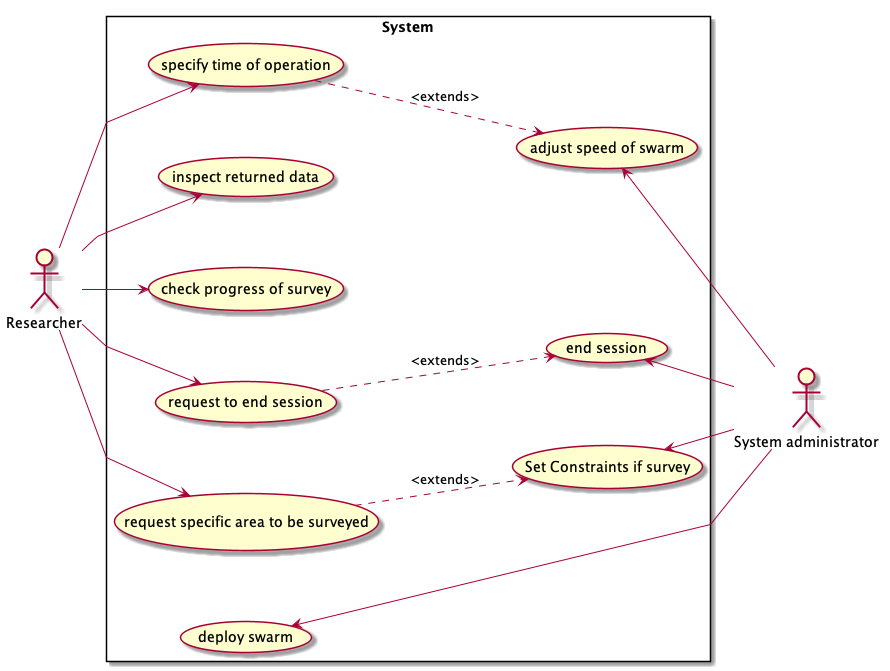
\includegraphics[width=\textwidth]{diagrams/usecase.png}
   \caption{Use Case Diagram}
   \label{fig:ucd}
\end{figure}
\subsection{Mandated Constraints}
There are 2 constraints put on the project. The first being time, since the project is due at the end of April 2019. The second constraint is money. There is a \$750 budget for this project.
\subsection{Undesired Behavior}
An insect should not lose connection to the server during the survey. An insect should not be hit or come in the path on any object including other insects. The power supply of an insect should not explode. The water should not interfere with the operations of an insect. Other network signals should not interfere with the server and the swarm. 
\subsection{Variables}
\begin{figure}[H]
   \centering
   \noindent\begin{tabularx}{\textwidth}{| >{\centering\arraybackslash}m{0.2\textwidth} | >{\centering\arraybackslash}m{0.2\textwidth} | >{\centering\arraybackslash}m{0.2\textwidth} | >{\centering\arraybackslash}m{0.285\textwidth} |}
   \hline 
   \textbf{Variable Name} & \textbf{Type} & \textbf{Value} & \textbf{Description} \\
   \hline
   Area of survey & Fixed & $X$ in $m^2$ & The total surface area of water in a survey \\ \hline
   Perimeter of survey & Fixed & $X$ in $m$ & The region that bounds the survey on a body of water \\ \hline
   \hyperref[sec:definitions]{Insect} location & Monitored & (X, Y) representing lat/lon values, respectively & The perceived location of an insect at any given time\\ \hline
   Temperature & Monitored & $X$ in $^\circ$C & The measurement an insect takes at a specific point\\ \hline
   Speed of  \hyperref[sec:definitions]{Insect} & Controlled & $X$ in $m/s$  & The speed relative to the water of an insect \\ \hline
   Number of \hyperref[sec:definitions]{Insect} & Controlled & $X$ amount of insects & The number insects currently deployed in a swarm\\ \hline
   Battery life & Monitored & $X$ in $minutes$ & The amount of battery left in a specific insect \\ \hline
   Range of communication & Fixed & $X$ in $m$ & The range in which server can communicate with each insect \\ \hline
   Max Time for survey & Fixed & $X$ in minutes & The maximum time the survey will run for\\ \hline
   Min Time for survey & Fixed & $X$ in minutes & The minimum time the survey will run for \\ \hline
   Start Point & Fixed & (X, Y) representing lat/lon values, respectively & The Starting point from where an insect is deployed \\ \hline
   \end{tabularx}
   \caption{List of Variables}
\end{figure}

\subsection{Context Diagram}
\begin{figure}[H]
   \centering
   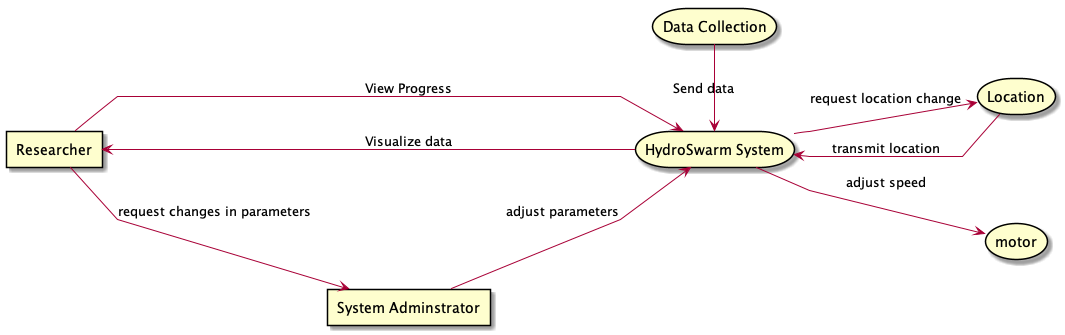
\includegraphics[width=\textwidth]{diagrams/context.png}
   \caption{Context Diagram}
   \label{fig:cd}
\end{figure}

\section{Functional Decomposition Diagram}
\begin{figure}[H]
   \centering
   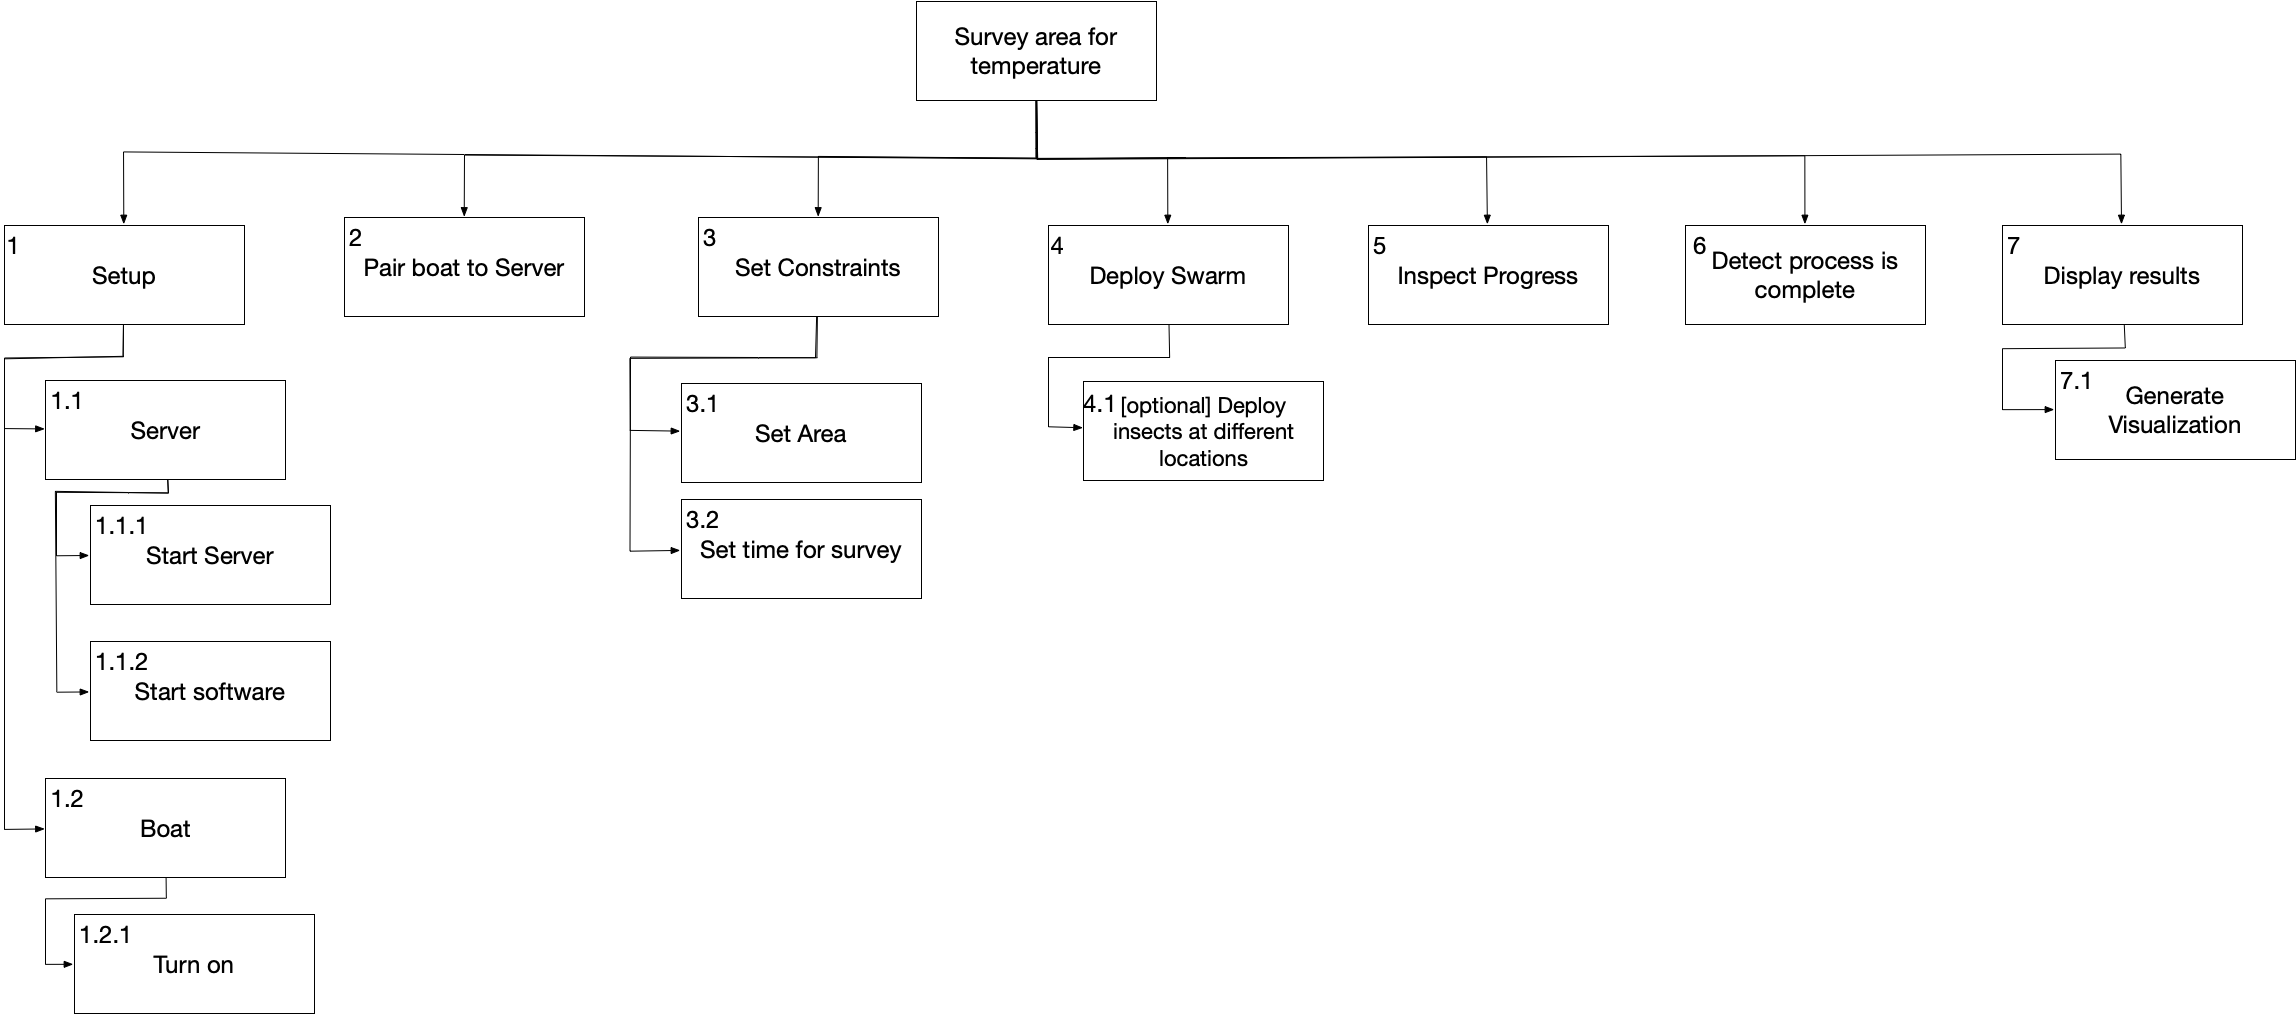
\includegraphics[width=\textwidth]{diagrams/functionaldecomp.png}
   \caption{Functional Decomposition Diagram}
   \label{fig:fdd}
\end{figure}

\section{Functional Requirements}

\functionalRequirement
{1}
{Each \hyperref[sec:definitions]{insect} in the
\hyperref[sec:definitions]{swarm}
must be able to measure
the water temperature at its current location}
{Accurate water temperature measurements have many applications
in academic or professional work}
{Each insect must be able to measure the water accuracy at its location
to within \pm $ 1^o C$ at all times}
{Victor Velechovsky}
{High}
{Created Oct. 28, 2018}

\functionalRequirement
{2}
{Each \hyperref[sec:definitions]{insect} in the
\hyperref[sec:definitions]{swarm}
must be able to provide its current location}
{Water temperature measurements must be combined with the location
at which they are measured}
{Each \hyperref[sec:definitions]{insect}'s location must be known to within
$1m$ accuracy at all times}
{Victor Velechovsky}
{High}
{Created Oct. 28, 2018}

\functionalRequirement
{3}
{The \hyperref[sec:definitions]{system} must be able to produce temperature
measurements, specified in Requirement F1, at many different locations
in a body of water}
{Producing many data points provides a more accurate representation of the
underlying property (in our case, the temperature of the water)}
{The \hyperref[sec:definitions]{system} must produce at least 5 different
measurements for each \hyperref[sec:definitions]{insect} that is
available}
{Victor Velechovsky}
{High}
{Created Oct. 28, 2018}

\functionalRequirement
{4}
{The \hyperref[sec:definitions]{system} must be able to produce a \hyperref[sec:definitions]{Water Temperature Map} of a swimming pool-sized body of water}
{Producing a visual temperature map of a body of water is a useful
tool for analyzing measurement data}
{The swarm must be able to produce a visualization that displays a representation
of the temperature measurement data}
{Victor Velechovsky}
{High}
{Created Oct. 28, 2018}

\functionalRequirement
{5}
{Each \hyperref[sec:definitions]{insect} in the \hyperref[sec:definitions]{system} shall be maneuverable such that it can move to any position (x, y) on the surface of the water}
{Allows proper coverage of the area of interest}
{The \hyperref[sec:definitions]{insect} is able to move to a specified position}
{Gabriel Potter}
{High}
{Created Oct. 31, 2018}

\functionalRequirement
{6}
{The \hyperref[sec:definitions]{system} shall be able to plan and control the paths of \hyperref[sec:definitions]{insect}s such that redundant measurements are not made and there are no collisions}
{Efficiency}
{There are no collisions (between insects) or redundant measurements}
{Gabriel Potter}
{High}
{Created Oct. 31, 2018}

\functionalRequirement
{7}
{The \hyperref[sec:definitions]{insect}s shall return to the start point when data collection is complete}
{Ease of use, cost effectiveness}
{All \hyperref[sec:definitions]{insect}s return when collection is complete}
{Gabriel Potter}
{High}
{Created Oct. 31, 2018}

\functionalRequirement
{8}
{The \hyperref[sec:definitions]{insect}s shall move in an autonomous manner}
{\hyperref[sec:definitions]{Swarm}s should move based on collective intelligence}
{All \hyperref[sec:definitions]{insect}s should move without control input from users}
{Nishanth Balamohan}
{High}
{Created Oct. 31, 2018}

\functionalRequirement
{9}
{If an \hyperref[sec:definitions]{insect} loses a critical function for autonomous operation (i.e. location) it shall have the ability to be manually overridden and controlled by the user}
{Allow the \hyperref[sec:definitions]{insect} to be easily returned to the start point}
{Each \hyperref[sec:definitions]{insect} has the ability to be manually controlled if the circumstances require it}
{Gabriel Potter}
{Medium}
{Created Oct. 31, 2018}

\functionalRequirement
{10}
{If an \hyperref[sec:definitions]{insect} loses critical functionality such as communication, sensing, or movement, the remaining operational \hyperref[sec:definitions]{insect}s should operate as if that \hyperref[sec:definitions]{insect} is no longer part of the swarm}
{A non-functional \hyperref[sec:definitions]{insect} provides no use to the \hyperref[sec:definitions]{swarm}}
{If an \hyperref[sec:definitions]{insect} fails to communicate or notifies the swarm of an error, the algorithm must recompute the paths based on the new number of \hyperref[sec:definitions]{insect}s}
{Nishanth Balamohan}
{High}
{Created Oct. 31, 2018}

\section{Non-Functional Requirements}

\subsection{Look and Feel Requirements}
\nonFunctionalRequirement
{1}
{The \hyperref[sec:definitions]{system}'s interface must look simple}
{Users want to use a simple interface}
{Users should be able to see all interface elements clearly and easily}
{Nishanth Balamohan}
{Low}
{Created Oct. 31, 2018}

\subsection{Usability and Humanity Requirements}

\nonFunctionalRequirement
{2}
{The \hyperref[sec:definitions]{system} shall have an interface with high learnability}
{Users want to interpret the data as fast as possible}
{Users should be able to understand the data that \hyperref[sec:definitions]{swarm} provide}
{Nishanth Balamohan}
{Low}
{Created Oct. 31, 2018}

\subsection{Performance Requirements}

\nonFunctionalRequirement
{3}
{The \hyperref[sec:definitions]{system} must collect data within a reasonable
maximum amount of time}
{Users do not want to wait too long for their results}
{The swarm must provide the measurement data with a latency (relative to the
time of measurement) of no more than $20s$}
{Victor Velechovsky}
{High}
{Created Oct. 28, 2018}

\nonFunctionalRequirement
{4}
{The \hyperref[sec:definitions]{system} must collect data for a long enough
amount of time without failing}
{Users want the system to collect data for long enough to produce enough
data points}
{The system must collect temperature measurements reliably for a minimum of
20m}
{Victor Velechovsky}
{High}
{Created Oct. 28, 2018}

\subsection{Operational and Environmental Requirements}

\nonFunctionalRequirement
{5}
{The \hyperref[sec:definitions]{swarm} must be able to work with an arbitrary
number of \hyperref[sec:definitions]{insects}}
{The number of boats in the swarm should be easily configurable}
{The swarm must work correctly with 3-30 insects}
{Victor Velechovsky}
{High}
{Created Oct. 29, 2018}

\nonFunctionalRequirement
{6}
{The \hyperref[sec:definitions]{server software} will run on Linux}
{Linux is a popular, efficient and well-supported operating system}
{The \hyperref[sec:definitions]{server software} will run on Linux}
{Victor Velechovsky}
{High}
{Created Oct. 30, 2018}

\nonFunctionalRequirement
{7}
{The user shall be able to pair \hyperref[sec:definitions]{insects}
to the server}
{Users should be able to pair as many insects as they want}
{Pairing must be easy to do}
{Victor Velechovsky}
{High}
{Created Oct. 30, 2018}

\subsection{Maintainability and Support Requirements}

\nonFunctionalRequirement
{8}
{The \hyperref[sec:definitions]{insects} will be waterproof in the areas that hold critical electronics}
{The electronics will fail and require replacement if they get wet}
{All critical areas are sufficiently waterproof}
{Gabriel Potter}
{High}
{Created Oct. 31, 2018}

\subsection{Security Requirements}

\nonFunctionalRequirement
{9}
{The project shall not allow unauthorized access of data}
{The user's data must be protected from unauthorized users}
{No unauthorized users should be granted access to user data}
{Nishanth Balamohan}
{Medium}
{Created Oct. 31, 2018}

\subsection{Political Requirements}

\nonFunctionalRequirement
{10}
{The project shall not use any text, images, or media that will
offend the users that purchase it}
{This project must not offend any users or cause any political conflicts}
{Any text, image, or media used should not cause offence to any user}
{Nishanth Balamohan}
{Medium}
{Created Oct. 31, 2018}

\subsection{Legal \& Compliance Requirements}

\nonFunctionalRequirement
{11}
{The project must comply with ethical standards}
{The project must be ethically responsible}
{The project must comply with the guidelines set by the Members Business \& Engineering Student Research Ethics Committee}
{Nishanth Balamohan}
{Medium}
{Created Oct. 31, 2018}

\subsection{Health and Safety Requirements}

\nonFunctionalRequirement
{12}
{The \hyperref[sec:definitions]{insects} will not travel too quickly}
{Fast moving boats may present a danger to the nearby environment}
{The boats will not travel faster than $10 km/h$}
{Victor Velechovsky}
{Medium}
{Created Oct. 29, 2018}

\nonFunctionalRequirement
{13}
{The \hyperref[sec:definitions]{insects} will not have exposed wiring}
{Expired wiring could be a safety concern to the nearby environment}
{The boats will not have any visible wiring under normal operation}
{Victor Velechovsky}
{Medium}
{Created Oct. 30, 2018}

\section{Project Issues}
\subsection{Open Issues}
Due to the complexity of the project, there are some open issues that our group might have to overcome to be successful. One of the open issues that we have is an error in data and how to check the validity of the temperature data received from the boats. For example, one of the insects in the swarm could potentially have a faulty reading and skew the data resulting in an invalid survey. Since our group has not chosen the temperature sensor yet, we do not have concrete information about the severity of this issue. Another open issue we have is the battery life for the insect. If it dies midway through the survey, it will result in missing data. In addition, if the insect battery dies, an issue that might arise is how to retrieve the insect and supplement the missing data. Path correction is also an open issue that might be difficult to solve since we do not have any information on direction or about the water current speed and location. 
\subsection{Off The Shelf Solutions}
In order to solve the open issues, some off-the-shelf solutions must be incorporated into the project. The error in temperature data, for example, can be solved by buying a more accurate temperature. However, the more accurate the temperature sensor, the higher the price, which is one of the constraints in this project. Another open issue that can be solved with Off The Shelf Solutions is the battery life. Again buying a larger battery will increase the life of the insect but will increase weight and costs which might affect other requirements. In addition, path correction might be solved by an accurate G.P.S. system but the price might force the solution to be too expensive to pursue. 
\subsection{New Problems}
As of October $30^{th}$ 2018, no new problems exist.
\subsection{Risk}
The largest risk that the group has is potentially going over budget. The cost will mainly be based on the number of insects we decide to build for the swarm. In addition, the precision of the sensors and motors used will also be correlated with price, which might increase as development progresses. 

\subsection{User Documentation \& Training}
The users will be informed of the following items in order to use the system efficiently:
\begin{itemize}
    \item Creating a boundary or area to survey
    \item Pairing insects with the server
    \item Limiting survey time
    \item Setting the number of insects in the swarm
    \item Deploying insects 
    \item How to read/interpret the resultant data
\end{itemize}
\end{document}
